\documentclass[12pt]{article}  % 12pt means font size
%\usepackage{CJKutf8}  % For Chinese typing
\usepackage{amsmath, amssymb, amsthm, mathrsfs}  % For mathematical symbols
\usepackage[a4paper, top=2.54cm, bottom=2.54cm, left=3.17cm, right=3.17cm]{geometry}  % This is the standard setting of thesis of NTHU. Do not change it.
\usepackage{rotating, booktabs}  % For table-rotating 
\usepackage{wallpaper}  % For watermark
%\CenterWallPaper{.18}{nthu-logo.jpg}  % Watermark of NTHU
%\usepackage{showlabels}  % When there are many equations in your thesis, it is a good tool to show them before printing the labels out. But remember comment it when you finish your thesis.
\numberwithin{equation}{subsection}
\linespread{1.5}  % The linespread is 1.5.
\newtheorem{thm}{Theorem}[section]  % Define new theorem.
\newtheorem{alg}{Algorithm}[section]  % Define new algorithm.
\newtheorem{lemma}[thm]{Lemma}
\newtheorem{conjecture}{Conjecture}[section]
\newtheorem{definition}[thm]{Definition}
\newtheorem{prop}{Proposition}[subsection]
\newtheorem*{rmk}{Remark}
\theoremstyle{plain}

\usepackage{xeCJK}
\setCJKmainfont[AutoFakeBold=5,AutoFakeSlant=.4]{標楷體}

\begin{document}
%\begin{CJK}{UTF8}{cwku}  % For Chinese typing

\begin{titlepage}  % Titlepage
\begin{center}
\huge 國立清華大學數學系應用數學組\\
\huge 碩士論文\\
\vspace*{15ex}
\huge Hardy空間的等價距之探討\\
\huge Quasi-norm Equivalence of Several Maximal Functions in Hardy space\\
\vspace*{10ex}

\begin{flushleft}
	\hspace{2cm}\LARGE 指導教授: 江金城 (Jin-Cheng Jiang)\\
	\hspace{2cm}\LARGE 研究生: 黃翊軒 (Yi-Hsuan Huang)\\
	\hspace{2cm}\LARGE 學號: 104021615\\
	\vspace*{3ex}
	
\end{flushleft}
\LARGE 中華民國一零六年七月
\end{center}
\end{titlepage}

\pagenumbering{roman}  % Use roman numbers before the main body.
\begin{center}
	\LARGE 摘要
\end{center}
本文探討Hardy上的多個等價半距,有時我們無法直接得出最大函數(maximal function)之間的距等價關係,可以先引進多個輔助函數,藉由輔助函數之間的大小關係來幫助我們得到原來函數之間所想要的結果
\newpage  % Independent page

\begin{abstract}  % Abstract
This thesis consists of two parts. In the first part, bla bla.

In the second part, bla bla.
\end{abstract}
\newpage  % Independent page

\begin{center}
\textbf{Acknowledgements}  % Acknowledgements
\end{center}
{\small

First of all, bla bla.

Last but not least, I am really indebted to my parents, bla bla.
}
\newpage

\tableofcontents  % Table of contents
\newpage
%\listoftables  % List of tables
%\newpage
%\listoffigures  % List of figures
%\newpage

\pagenumbering{arabic}  % Use arabic numbers when the main body starts.
\section{Introduction}  % You can rename the section title.
Hardy space $H^p(\mathbb{R}^n)$, $0<p<\infty$ are spaces of distribution have remarkable similarities to $L^p$. There exists an abundance of equivalent characterizations for Hardy spaces. The major objective of this study was to investigate one of the characterizations from historical views.

The organization of the thesis is the following. In Section 2, we provide a introduction to definition of Hardy space and serveral kinds of maximal functions needed to construct the desired characterization.

In Section 3, we introduce main theorem that all the maximal functions of the section 1 have comparable $L^p$ quasi-norms for all $0<p<\infty$. 
% You can cite the reference by using the command "\cite{}", "B" is the label you set up in the section of reference.

\section{Settings and Definitions}
In this section, we introduce definitions we would use in the later sections. First, we need some background to give the definition of Hardy space. We say that a tempered distribution $v$ is \textit{bounded} if $\varphi * v \in L^{\infty}(\mathbb{R}^n)$ whenever $\varphi$ is in Schwartz spaces $\mathcal{S}(\mathbb{R}^n)$.

We observe that if $v$ is a bounded tempered distribution and $h \in L^1(\mathbb{R}^n)$, then the convolution $h∗v$ can be defined as a distribution via the convergent integral $$\langle h*v,\varphi\rangle = \langle\tilde{\varphi}*v,\tilde{h}\rangle = \int_{\mathbb{R}^n} (\tilde{\varphi}*v)(x)(\tilde{h})(x)dx,$$ where $\varphi$ is a Schwartz function and $\tilde{\varphi}(x) = \varphi(-x)$, $\tilde{h}(x) = h(-x)$.

\subsection{Definition of Hardy Spaces}
\begin{definition}
	Let $f$ be a bounded tempered distribution on $\mathbb{R}^n$ and let $0<p<\infty$. We say that $f$ lies in the Hardy space $H^p(\mathbb{R}^n)$ if the Poisson maximal function $P(x)$
	\begin{align}
	M(f;P)(x) = \sup_{t>0}|(P_t*f)(x)| 
	\end{align}
	lies in $L^p(\mathbb{R}^n)$. If this is the case, we set $$\|f\|_{H^p} = \|M(f;P)(x)\|_{L^p}.$$ 
\end{definition}
	
\subsection{Definition of Several Maximal Functions}
Let $a,b > 0$. Let $\varPhi$ be a Schwartz function and let $f$ be a tempered distribution on $\mathbb{R}^n$. We define following maximal functions of $f$ with respect to $\varPhi$.
\begin{definition}[Smooth Maximal Function]
	The smooth maximal function of $f$ with respect to $\varPhi$ is defined as $$M(f;\varPhi)(x) = \sup_{t>0}|(\varPhi_t*f)(x)|$$ 
\end{definition}

\begin{definition}[Nontangential Maximal Function]
	 The nontangential maximal function (with aperture a) of f with respect to $\varPhi$ is defined as $$M_a^*(f;\varPhi)(x) = \sup_{t>0}\sup_{\substack{y\in \mathbb{R}^n\\ |y-x|\le at}}|(\varPhi_t*f)(x)|$$
\end{definition}

\begin{definition}[Auxiliary Maximal Function]
	The auxiliary maximal function is defined as $$M_b^{**}(f;\varPhi)(x) = \sup_{t>0}\sup_{y \in \mathbb{R}^n}\frac{|(\varPhi_t*f)(x-y)|}{(1+t^{-1}|y|)^b}$$
\end{definition}

Note that we have 
\begin{align}
M(f;\varPhi)(x) \le M_a^*(f;\varPhi)(x) \le (1+a)^bM_b^{**}(f;\varPhi)(x),
\end{align}
where the first inequilty is quickly from definitions and the second from viewing $M_b^{**}(f;\varPhi)(x) = \sup_{t>0}\sup_{y \in \mathbb{R}^n}\frac{|(\varPhi_t*f)(y)|}{(1+t^{-1}|x-y|)^b} $ and then restricting $|x-y| \le at$.

Finally, we also need to estimate the quantity of a Schwartz function.
\begin{definition}
	$$\mathfrak{N}_N(\varphi) = \int_{\mathbb{R}^n}(1+|x|)^N\sum_{|\alpha|\le N+1}|\partial^\alpha\varphi(x)|dx$$
\end{definition}

\begin{definition}[Grand Maximal Function]
	The grand maximal function of f (with respect to N) as $$\mathcal{M}_N(f)(x) = \sup_{\varphi \in \mathcal{F}_N}M_1^*(f;\varphi)(x)$$
\end{definition}

\section{Quasi-norm Equivalence of Sever Maximal Function}
Before stating the main theorem, we first introduce the following Lemma.
\subsection{Lemma}
\begin{lemma}
	Let $m \in \mathbb{Z}^+$ and let $\varPhi$ in $\mathcal{S}(\mathbb{R}^n)$ satisfy $\int_{\mathbb{R}^n}\varPhi(x)dx = 1$, Then there exists a constant $C_0(\varPhi, m)$ such that for any $\varPsi$ in $\mathcal{S}(\mathbb{R}^n)$, there are Schwartz functions $\varTheta^{(s)}$, $0\le s\le 1$, with the properties
	\begin{align}
		\varPsi(x) = \int_{0}^{1}(\varTheta^{(s)}*\varPhi_s)(x)ds \label{lemma}
	\end{align}
	and
	\begin{align}
		\int_{\mathbb{R}^n}(1+|x|)^m\left| \varTheta^{(s)}(x) \right| dx \le C_0(\varPhi, m)s^m\mathfrak{N}_m(\varPsi)
	\end{align}
\end{lemma}
\begin{proof}
	We start with a smooth function $\zeta$ supported in $[0,1]$ that satisfies
	\begin{align*}
		0\le \zeta &\le \frac{2s^m}{m!} \qquad \text{for all } 0\le s \le 1 \\ 
		\zeta(s) &= \frac{s^m}{m!} \qquad \text{ for all } 0 \le s \le \frac{1}{2} \\
		\frac{d^r\zeta}{dt^r}(1) &= 0 \qquad \quad \text{ for all } 0\le r \le m+1 \\
	\end{align*}
	We define
	\begin{align}
		\varTheta^{(s)} = \varXi^{(s)} - \frac{d^{m+1}\zeta}{ds^{m+1}}(s) \left( \stackrel{\text{m+1 terms}}{\overbrace{\varPhi_s* \cdots *\varPhi_s}}\right) * \varPsi,
	\end{align}
	where
	\begin{align*}
		\varXi^{(s)} = (-1)^{m+1}\zeta(s)\frac{d^{m+1}\zeta}{ds^{m+1}}\left( \stackrel{\text{m+2 terms}}{\overbrace{\varPhi_s* \cdots *\varPhi_s}}\right) * \varPsi,
	\end{align*}
	and we claim that (\ref{lemma}) holds for this choice of $\varTheta^{(s)}$. To verify this assertion, we apply integration by parts to write
	\begin{align*}
		\int_{0}^{1}-\frac{d^{m+1}\zeta}{ds^{m+1}}(s)( \stackrel{\text{m+2 terms}}{\overbrace{\varPhi* \cdots *\varPhi}})_s * \varPsi ds = -\stackrel{=0}{\overbrace{\frac{d^m\zeta}{ds^m}(1)}}( \stackrel{\text{m+2 terms}}{\overbrace{\varPhi* \cdots *\varPhi}})_1 * \varPsi \\
		+\stackrel{=1}{\overbrace{\frac{d^m\zeta}{ds^m}(0)}}\lim_{s\rightarrow 0^+}( \stackrel{\text{m+2 terms}}{\overbrace{\varPhi* \cdots *\varPhi}})_s*\varPsi\\
		+\int_{0}^{1}\frac{d^m\zeta}{ds^m}(s)\frac{d}{ds}( \stackrel{\text{m+2 terms}}{\overbrace{\varPhi* \cdots *\varPhi}})_s*\varPsi ds
	\end{align*}
	Therefore appling $m+1$ times integration by parts we rewrite (\ref{lemma}) as 
	\begin{align*}
		\int_{0}^{1}\varTheta^{(s)}*\varPsi_sds = \int_{1}^{0}\varXi^{(s)}*\varPsi_sds + \frac{d^{m}\zeta}{ds^{m}}(0)\lim_{s\rightarrow 0^+}( \stackrel{\text{m+2 terms}}{\overbrace{\varPhi* \cdots *\varPhi}})_s*\varPsi\\
		-(-1)^{m+1}\int_{0}^{1}\zeta(s)\frac{d^{m+1}}{s^{m+1}}\left( \stackrel{\text{m+2 terms}}{\overbrace{\varPhi_s* \cdots *\varPhi_s}}\right) * \varPsi ds.
	\end{align*}
	Noting that all the boundary terms vanish except for the term at $s = 0$ in the first integration by parts. The first and the third terms in the previous expression on the right add up to zero, while the second term is equal to $\varPsi$, since $\varPsi$ has integral one. This implies that the family $\{(\varPhi*\cdots*\varPhi)_s\}_{s>0}$ is an appproximate identity as $s \rightarrow 0^+$. Specifically, from $\|\varPhi*\varPhi\|_1 \le \|\varPhi\|_1\|\varPhi\|_1 = 1$ and $\int_{\mathbb{R}^n}\varPhi dx = \int_{\mathbb{R}^n}\varPhi_s dx = 1$, we have
	$$	
	\int_{\mathbb{R}^n}(\varPhi*\cdots*\varPhi)_s dx = 1
	$$
	Since $\varPsi \in L^{\infty}(\mathbb{R}^n)$, appling the statement from Zygmund's real analysis textbook
	\begin{thm}
		Let $f_{\varepsilon} = f*K_{\varepsilon}$, where $K\in L^1(\mathbb{R}^n)$ and $\int_{\mathbb{R}^n}K = 1$. If $f \in L^{\infty}(\mathbb{R}^n)$, then $f_{\varepsilon}\rightarrow f$ as $\varepsilon \rightarrow 0$ at every point of continuity of f, and the convergence is uniform on any set where f is uniformly continuous.
	\end{thm}
	Therefore, the lemma follows.
\end{proof}
分隔線





%\subsection{Basic Monte Carlo Simulations}
%As a computational method, Monte Carlo method relies on reiterating sampling random variables in a specific domain. In that, bla bla.
%\begin{alg}  % The new algorithm I defined by myself.
%\begin{itemize}  % The way to itemize. Another way is to replace "itemize" with "enumerate".
%(Basic Monte Carlo Simulations)
%\item Step 1: Bla bla.
%\item Step 2: Bla bla.
%\end{itemize}
%\end{alg}

%Given an estimator $\bar{x}$ as the average from the sample space $X$. Bla bla.
% You can put some mathematical symbols between "$" and "$".


\subsection{Importance Sampling Method}
Even with the aid of ever faster computers nowadays, the slow convergence speed is still the limit of basic Monte Carlo simulations. Bla bla.

\begin{align}
\mathbb{P}\left\lbrace X>c\right\rbrace \label{MCP}
\end{align}
% You can put equations between "\begin{align}" and "\end{align}", or "\[" and "\]".
% If you don't want the labels behind the equations, just replace "align" with "align*".
% Another way is to put the command "\notag" after the equations. Just like the next equations.
% "\label{}" is the command that you can name the equation.

\begin{align}
\mathbb{P}\left\lbrace X>c\right\rbrace&=\mathbb{\tilde{E}}\left[ \mathbb{I}_{\left\lbrace X>c\right\rbrace }\right]  \notag\\
&=\mathbb{E}\left[ \mathbb{I}_{\left\lbrace Y>c\right\rbrace }e^{\frac{c^2}{2}-cY}\right] \label{ISP}
\end{align}
% Put "&" before "=" can align the "=".
where $Y\sim N(c,1)$. And Equation (\ref{ISP}) is more easier to sample the rare events than the original one.
% "\ref{}" is the command that you can cite the equations you named before.


\section{Pricing Contingent Claims}
In this section, we will discuss bla bla.

\subsection{European Options}
European options are the fundamental options. As a result, they are also called ``vanilla" or ``plain" options.
% Note that it is the right way to type the quotation marks in English.

\subsubsection{Proof of Efficiency of Importance Sampling}
In this section, we will prove that our importance sampling methods are bla bla.

\begin{thm}  % The new theorem I defined by myself.
If the following approximation holds, for large c
\[
\mathbb{E}\left[ \left( \mathbb{I}_{\left\lbrace Z>c\right\rbrace }e^{\frac{c^2}{2}-cZ}\right) ^2\right] \approx p^2,
\]
then bla bla.
\end{thm}

\begin{proof}  % Proof. No need to define in advance.

\begin{align}
q={}& \mathbb{E}\left[ e^{-2rT}S_0^2e^{2\left( r-\frac{\sigma^2}{2}\right) T+2\sigma\sqrt{T}Z}\mathbb{I}_{\left\lbrace Z>c\right\rbrace }e^{\alpha^2-2\alpha Z}\right] \notag\\
&-2K\mathbb{E}\left[ e^{-2rT}S_0e^{\left( r-\frac{\sigma^2}{2}\right) T+\sigma\sqrt{T}Z} \mathbb{I}_{\left\lbrace Z>c\right\rbrace }e^{\alpha^2-2\alpha Z}\right] \notag\\
&+K^2\mathbb{E}\left[ e^{-2rT}\mathbb{I}_{\left\lbrace Z>c\right\rbrace }e^{\alpha^2-2\alpha Z}\right] \notag\\
={}&S_0^2\mathbb{E}\left[ \mathbb{I}_{\left\lbrace Z>c\right\rbrace }e^{-\sigma^2 T+\alpha^2-(2\alpha-2\sigma\sqrt{T})Z}\right] \notag\\
&-2S_0Ke^{-rT}\mathbb{E}\left[ \mathbb{I}_{\left\lbrace Z>c\right\rbrace }e^{-\frac{\sigma^2}{2}T+\alpha^2-(2\alpha-\sigma\sqrt{T})Z}\right] \notag\\
&+K^2e^{-2rT}\mathbb{E}\left[ \mathbb{I}_{\left\lbrace Z>c\right\rbrace }e^{\alpha^2-(2\alpha) Z}\right] \notag\\
={}&S_0^2e^{-\alpha^2+4\alpha\sigma\sqrt{T}-3\sigma^2 T}\mathbb{E}\left[ \mathbb{I}_{\left\lbrace Z>c\right\rbrace }e^{\frac{(2\alpha-2\sigma\sqrt{T})^2}{2}-(2\alpha-2\sigma\sqrt{T})Z}\right] \notag\\
&-2S_0Ke^{-rT}e^{-\alpha^2+2\alpha\sigma\sqrt{T}-\sigma^2 T}\mathbb{E}\left[ \mathbb{I}_{\left\lbrace Z>c\right\rbrace }e^{\frac{(2\alpha-\sigma\sqrt{T})^2}{2}-(2\alpha-\sigma\sqrt{T})Z}\right] \notag\\
&+K^2e^{-2rT}e^{-\alpha^2}\mathbb{E}\left[ \mathbb{I}_{\left\lbrace Z>c\right\rbrace }e^{\frac{(2\alpha)^2}{2}-(2\alpha) Z}\right] \notag\\
={}&S_0^2e^{-\alpha^2+4\alpha\sigma\sqrt{T}-3\sigma^2 T}e^{2\alpha^2-6\alpha\sigma\sqrt{T}}\mathbb{E}^{(1)}\left[ \mathbb{I}_{\left\lbrace Z^{(1)}>c\right\rbrace }\right] \notag\\
&-2S_0Ke^{-rT}e^{-\alpha^2+2\alpha\sigma\sqrt{T}-\sigma^2 T}e^{2\alpha^2-3\alpha\sigma\sqrt{T}}\mathbb{E}^{(2)}\left[ \mathbb{I}_{\left\lbrace Z^{(2)}>c\right\rbrace }\right] \notag\\
&+K^2e^{-2rT}e^{-\alpha^2}e^{2\alpha^2}\mathbb{E}^{(3)}\left[ \mathbb{I}_{\left\lbrace Z^{(3)}>c\right\rbrace }\right] \notag\\
={}&S_0^2e^{\alpha^2-2\alpha\sigma\sqrt{T}-3\sigma^2 T}\mathbb{E}^{(1)}\left[ \mathbb{I}_{\left\lbrace \tilde{Z}>c+\alpha-2\sigma\sqrt{T}\right\rbrace }\right] \notag\\
&-2S_0Ke^{-rT}e^{\alpha^2-\alpha\sigma\sqrt{T}-\sigma^2 T}\mathbb{E}^{(2)}\left[ \mathbb{I}_{\left\lbrace \tilde{Z}>c+\alpha-\sigma\sqrt{T}\right\rbrace }\right] \notag\\
&+K^2e^{-2rT}e^{\alpha^2}\mathbb{E}^{(3)}\left[ \mathbb{I}_{\left\lbrace \tilde{Z}>c+\alpha\right\rbrace }\right] \notag\\
={}&S_0^2e^{\alpha^2-2\alpha\sigma\sqrt{T}-3\sigma^2 T}N\left( -c-\alpha+2\sigma\sqrt{T}\right) \notag\\
&-2S_0Ke^{-rT}e^{\alpha^2-\alpha\sigma\sqrt{T}-\sigma^2 T}N\left( -c-\alpha+\sigma\sqrt{T}\right) \notag\\
&+K^2e^{-2rT}e^{\alpha^2}N\left( -c-\alpha\right) \label{op0}
\end{align}
% I reserve the proof in order to show how to handle the long equations.
\end{proof}

\subsubsection{Numerical Results}

\begin{sidewaystable}  % The way to handle long table. Just rotate it.
\begin{center}
\begin{tabular}{cccccccc}\toprule
\  & BS Formula & \multicolumn{2}{c}{Method 1 (Separation)} & \multicolumn{2}{c}{Method 2 (Final Stock Price)} & \multicolumn{2}{c}{Method 3 (Whole Stock Path)} \\ \midrule
$S_0$ & BS & MC(SE) & IS(SE) & MC(SE) & IS(SE) & MC(SE) & IS(SE)\\ \midrule
20 & 0.0002 & 0.0000(0.0000) & 0.0002(0.0000) & 0.0000(0.0000) & 0.0002(0.0000) & 0.0008(0.0008) & 0.0002(0.0000) \\
30 & 0.0120 & 0.0129(0.0057) & 0.0122(0.0002) & 0.0201(0.0071) & 0.0117(0.0002) & 0.0092(0.0035) & 0.0120(0.0002) \\
40 & 0.1307 & 0.1394(0.0206) & 0.1317(0.0015) & 0.1390(0.0200) & 0.1268(0.0017) & 0.1258(0.0188) & 0.1303(0.0017) \\
50 & 0.6201 & 0.5491(0.0422) & 0.6247(0.0070) & 0.5723(0.0426) & 0.6257(0.0080) & 0.6318(0.0493) & 0.6119(0.0080) \\
60 & 1.8442 & 1.7626(0.0818) & 1.8543(0.0206) & 1.8550(0.0881) & 1.8468(0.0243) & 2.0688(0.1002) & 1.8530(0.0244) \\
70 & 4.1112 & 4.1254(0.1347) & 4.1390(0.0474) & 4.2075(0.1330) & 4.1501(0.0580) & 4.1799(0.1376) & 4.2504(0.0581) \\
80 & 7.5782 & 7.6457(0.1959) & 7.5930(0.0940) & 7.4929(0.1902) & 7.5067(0.1162) & 7.6309(0.1947)& 7.5453(0.1164) \\
90 & 12.2497 & 12.4345(0.2561) & 12.4287(0.1698) & 12.6012(0.2548) & 12.5674(0.2162) & 12.4271(0.2575) & 12.1825(0.2098) \\
100 & 18.0230 & 17.9212(0.3132) & 17.9249(0.2855) & 18.0691(0.3130) & 18.0856(0.3645) & 17.8826(0.3122) & 18.3281(0.3754) \\
110 & 24.7413 & 24.5990(0.1470) & 24.6509(0.1241) & 25.0272(0.1516) & 24.9238(0.1018) & 24.8550(0.1507) & 24.6892(0.1014) \\
120 & 32.2343 & 32.3142(0.1313) & 32.2657(0.0882) & 32.3424(0.1305) & 32.3059(0.0728) & 32.4487(0.1339) & 32.1958(0.0729) \\
130 & 40.3420 & 40.2426(0.1123) & 40.3097(0.0628) & 40.4034(0.1154) & 40.2937(0.0525) & 40.2442(0.1126) & 40.4022(0.0526) \\
140 & 48.9259 & 48.8750(0.0982) & 48.8083(0.0453) & 48.9334(0.0987) & 48.9342(0.0388) & 48.9562(0.0973) & 48.9011(0.0388) \\
150 & 57.8728 & 57.8214(0.0827) & 57.8653(0.0334) & 57.8235(0.0843) & 57.8834(0.0287) & 57.8361(0.0842) & 57.9287(0.0287) \\
160 & 67.0929 & 67.0749(0.0716) & 67.0902(0.0247) & 67.2048(0.0737) & 67.0782(0.0213) & 66.9499(0.0680) & 67.0564(0.0215) \\
170 & 76.5166 & 76.4533(0.0610) & 76.5135(0.0182) & 76.4662(0.0604) & 76.4883(0.0160) & 76.4513(0.0598) & 76.5503(0.0161) \\
180 & 86.0915 & 86.1164(0.0525) & 86.0737(0.0136) & 86.1268(0.0528) & 86.0918(0.0122) & 86.0650(0.0528) & 86.0856(0.0121) \\ \bottomrule
\end{tabular}
\caption[Results of European Option Pricing]{Results of European Option Pricing: $S_0$ is underlying's initial price; BS is the price computed under BS model; Method 1, 2, 3 are we mentioned previously respectively, it consist of the results of basic Monte Carlo and importance sampling.}
\end{center}
\end{sidewaystable}
\newpage
% You can put description in "\caption[]", and it would be shown in the list of tables. 

\subsection{European Options with Stochastic Volatility}

In these two model, bla bla.

\subsubsection{Basic Monte Carlo Simulations}

First, we focus on the Vasicek model, we define it as the following,
\[
\left\{
\begin{array}{ll}
dS_t= rS_tdt+e^{\frac{y_t}{2}}d\tilde{W}_{1t}\\
dy_t=\alpha\left( m-y_t\right) dt+\beta d\tilde{Z}_{2t}
\end{array} \right.
\]
% The way to show big parentheses.

\subsubsection{Numerical Results}
% The normal table.
\begin{table}[h]
\begin{center}
\begin{tabular}{cccc}\toprule
\ & \multicolumn{3}{c}{Heston Model} \\ \midrule
$S_0$ & MC(SE) & IS(SE) & SE Reduction \\ \midrule
20 & 0.1525(0.0291) & 0.1384(0.0023) & 12.6387 \\
30 & 0.6013(0.0771) & 0.6554(0.0101) & 7.6525 \\
180 & 89.2501(0.1445) & 89.1496(0.0672) & 2.1513 \\ \bottomrule
\end{tabular}
\caption[Results of European Option Pricing with Stochastic Volatility and Interest Rate]{Results of European Option Pricing with Stochastic Volatility and Interest Rate: $S_0$ is underlying's initial price; Heston model is what we mentioned previously, it consist of the results of basic Monte Carlo and importance sampling.}
\end{center}
\end{table}

\section{Fourier Series Method}
The second and the main topic of this thesis begins, bla bla.

\subsection{Example}
Figure \ref{FV} shows the results of our example. And meantime, the sum of absolute error of the simulated example is shown next.
\begin{figure}[h]  % Put pictures here.
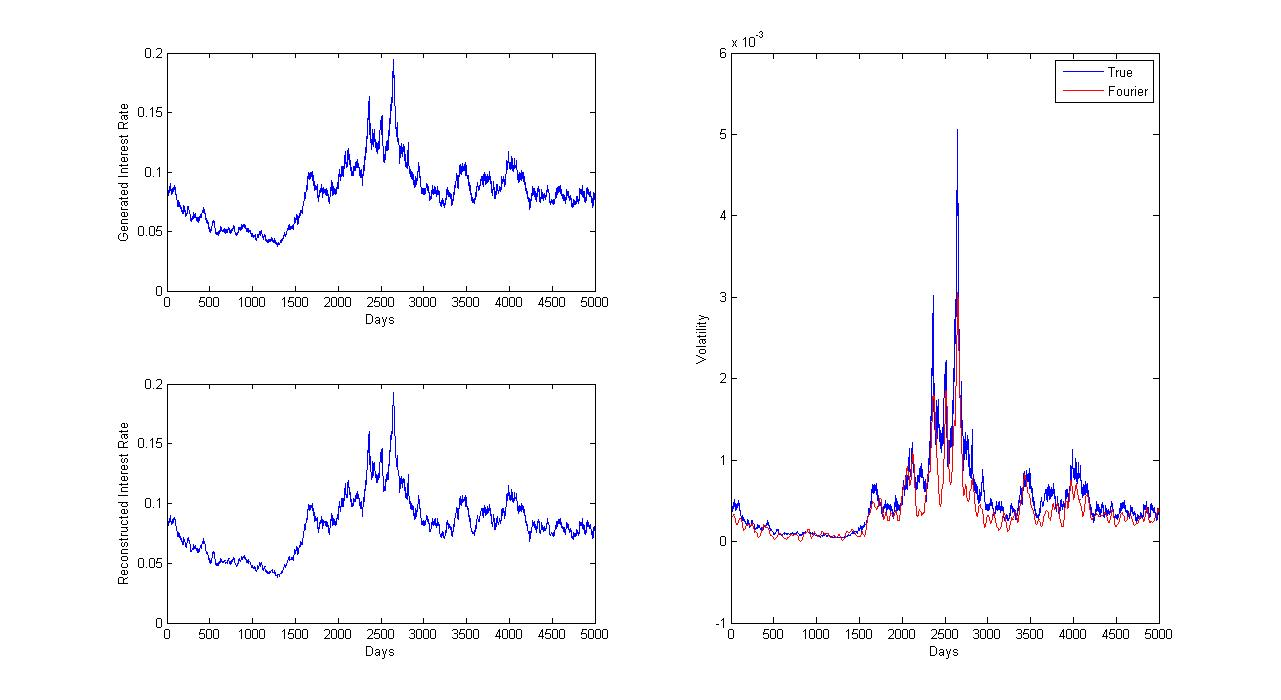
\includegraphics[width=15cm]{Fourier_Vasicek.jpg}
\caption{Estimate Volatility Process of Simulated Interest Rate by Fourier Series Method} \label{FV}
\end{figure}

\section{Conclusions}
We have done with option pricing and its inverse problem, model calibration, so far. Bla bla.

To sum up, bla bla.
\newpage

\begin{thebibliography}{99}  % The section of reference
\addcontentsline{toc}{section}{Reference}  % Add "Reference" into the table of contents
\bibitem{B}  % "B" is what you want to call it, and you need the name when citing it.
Bolye, P. (1977), ``Options: A Monte Carlo Approach". \emph{Journal of Financial Economics}, 4, 323-338
\bibitem{Shreve}
Shreve, S. (2004), ``Stochastic Calculus for Finance II: Continuous-Time Models". \emph{Springer}
\end{thebibliography}
\newpage

\addcontentsline{toc}{section}{Appendix}  % The section of appendix and add it into the table of contents
\appendix

%\end{CJK}
\end{document} 